\chapter{Meta}
\section{Vorgeschichte}
Im Oktober 2021 wurde es langsam Zeit ein Thema für unsere Diplomarbeit zu finden. Anfangs
hatten wir nur die Idee eine App zu entwickeln, jedoch fehlte uns die passende Inspiration. Philipp
wandte sich mit diesem Problem an Herr Professor Vogt, welcher direkt nach unseren privaten
Interessen fragte. Er meinte, es wäre viel einfacher und motivierender an einem Projekt zu arbeiten,
welches einen auch selbst interessiert.

Wir sind leidenschaftliche Skateboarder und hatten anfangs Probleme damit, umliegende Parks
zu finden oder neue Skater-Kollegen kennenzulernen. Somit haben wir uns entschlossen eine
App bzw. eine Website zu entwickeln, die Anfängern das Leben erleichtern soll.

\section{Projektlogo}
\label{logo}

Auf dem Logo ist ein Skateboard zu sehen, welches durch ein Portal aus einem Smartphone fliegt.
Der Designer des Logos ließ sich vom Portal aus der Serie \textit{Rick and Morty} inspirieren und wollte damit die Verbindung zwischen
der Technik und dem Sport zum Ausdruck bringen.

\begin{figure}[H]
    \centering
    \hfill
    \subfigure[Rick and Morty Staffel 1 Werbebild~\cite{rickAndMortySeason1}]{\includegraphics[height=0.4\textwidth]{images/Intro/RnM_S1.jpg}}
    \hfill
    \subfigure[SkateBuddy Projektlogo]{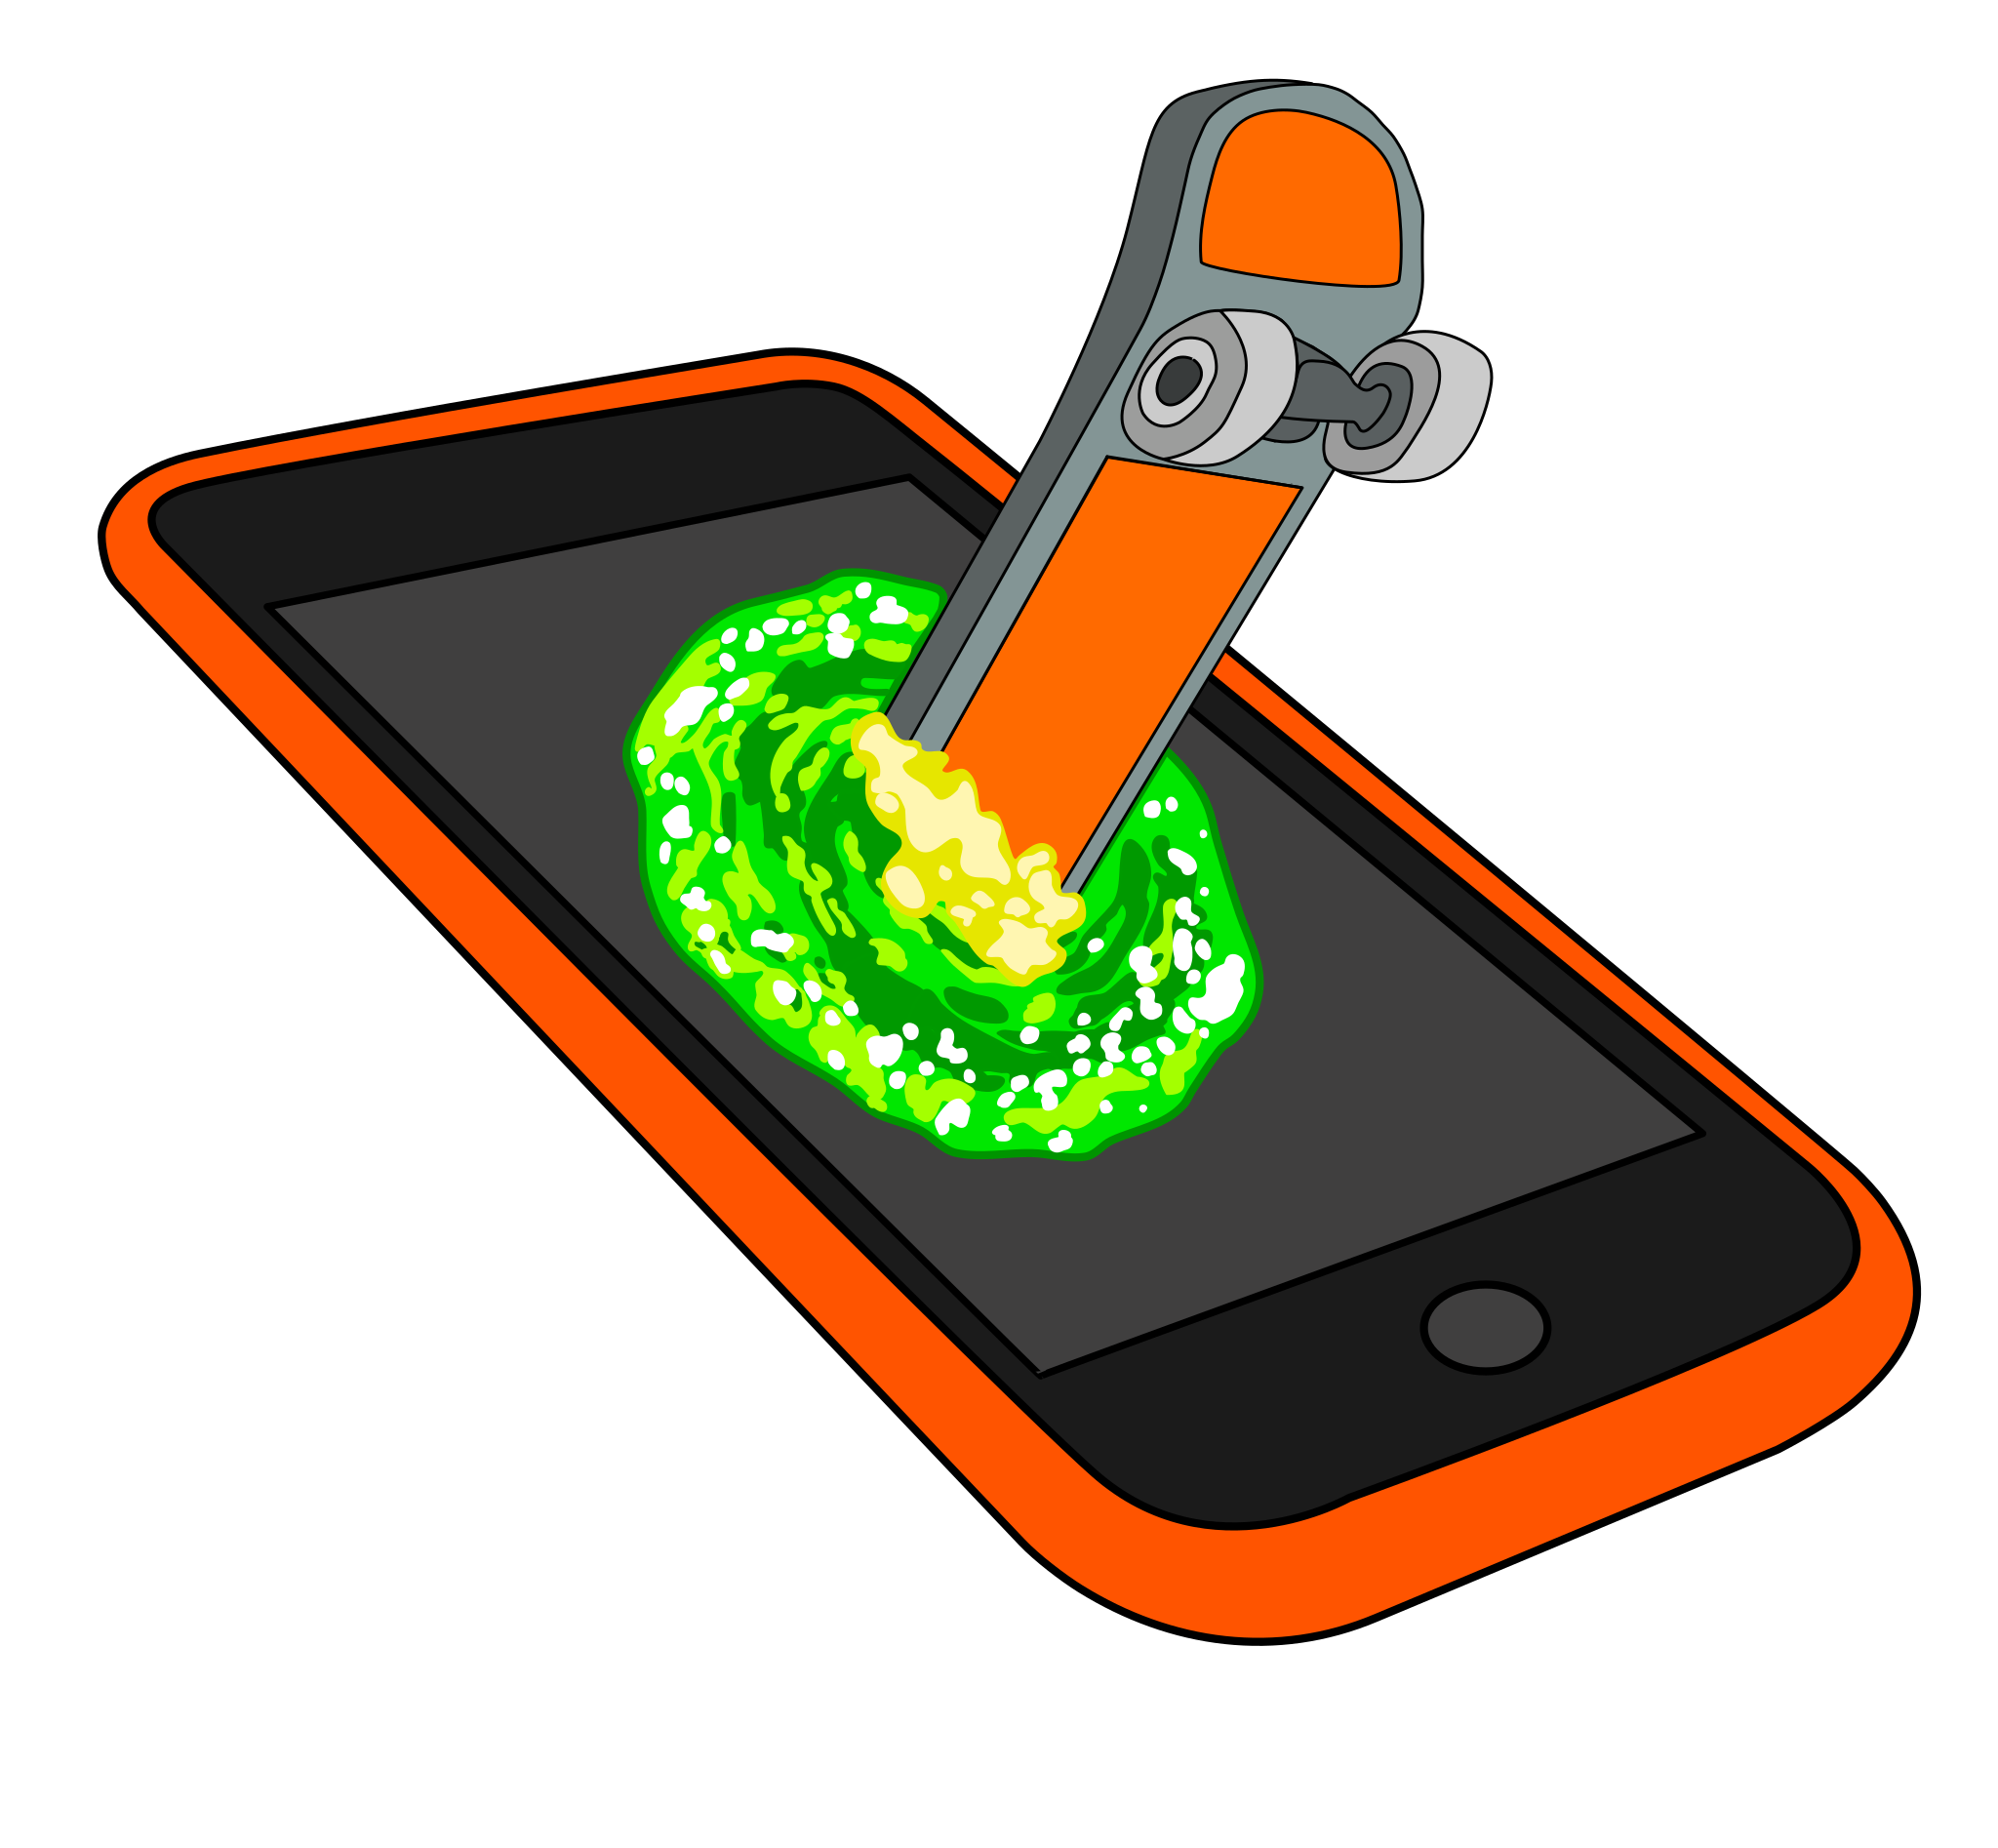
\includegraphics[width=0.4\textwidth]{images/logo.png}}
    \hfill
    \caption{Vergleich zwischen Portal aus der Serie und dem Logo}
\end{figure}